\documentclass{article}

\usepackage{tikz} 
\usetikzlibrary{automata, positioning, arrows} 

\usepackage{amsthm}
\usepackage{amsfonts}
\usepackage{amsmath}
\usepackage{amssymb}
\usepackage{fullpage}
\usepackage{color}
\usepackage{parskip}
\usepackage{hyperref}
  \hypersetup{
    colorlinks = true,
    urlcolor = blue,       % color of external links using \href
    linkcolor= blue,       % color of internal links 
    citecolor= blue,       % color of links to bibliography
    filecolor= blue,        % color of file links
    }
    
\usepackage{listings}

\definecolor{dkgreen}{rgb}{0,0.6,0}
\definecolor{gray}{rgb}{0.5,0.5,0.5}
\definecolor{mauve}{rgb}{0.58,0,0.82}

\lstset{frame=tb,
  language=haskell,
  aboveskip=3mm,
  belowskip=3mm,
  showstringspaces=false,
  columns=flexible,
  basicstyle={\small\ttfamily},
  numbers=none,
  numberstyle=\tiny\color{gray},
  keywordstyle=\color{blue},
  commentstyle=\color{dkgreen},
  stringstyle=\color{mauve},
  breaklines=true,
  breakatwhitespace=true,
  tabsize=3
}

\newtheoremstyle{theorem}
  {\topsep}   % ABOVESPACE
  {\topsep}   % BELOWSPACE
  {\itshape\/}  % BODYFONT
  {0pt}       % INDENT (empty value is the same as 0pt)
  {\bfseries} % HEADFONT
  {.}         % HEADPUNCT
  {5pt plus 1pt minus 1pt} % HEADSPACE
  {}          % CUSTOM-HEAD-SPEC
\theoremstyle{theorem} 
   \newtheorem{theorem}{Theorem}[section]
   \newtheorem{corollary}[theorem]{Corollary}
   \newtheorem{lemma}[theorem]{Lemma}
   \newtheorem{proposition}[theorem]{Proposition}
\theoremstyle{definition}
   \newtheorem{definition}[theorem]{Definition}
   \newtheorem{example}[theorem]{Example}
\theoremstyle{remark}    
  \newtheorem{remark}[theorem]{Remark}

\setcounter{tocdepth}{3}  % This makes subsubsections (level 3) appear in TOC
\setcounter{secnumdepth}{3}  % This makes subsubsections numbered
  

\title{CPSC-354 Report}
\author{Your Name  \\ Chapman University}

\date{\today} 

\begin{document}

\maketitle

\begin{abstract}
This is the place to write an abstract. The abstract should be a short summary of the report. It should be written in a way that makes it possible to understand the purpose of the report without reading it. You can write a dummy abstract first and replace it with a real one later in the semester.
\end{abstract}

\setcounter{tocdepth}{3}
\tableofcontents

\section{Introduction}\label{intro}

This report will document your learning throughout the course. It will be a collection of your notes, homework solutions, and critical reflections on the content of the course. Something in between a semester-long take home exam and your own lecture notes.\footnote{One purpose of giving the report the form of lecture notes is that self-explanation is a technique proven to help with learning, see Chapter 6 of Craig Barton, How I Wish I'd Taught Maths, and references therein. In fact, the report can lead you from self-explanation (which is what you do for the weekly deadline) to explaining to others (which is what you do for the final submission). Another purpose is to help those of you who want to go on to graduate school to develop some basic writing skills. A report that you could proudly add to your application to graduate school (or a job application in industry) would give you full points.}

To write your own report, you start from \texttt{report.tex} which is available in the course repo. For guidance on how to do this read on and also consult \texttt{latex-example.tex} which is also available in the repo. Also check out the usual resources (Google, Stackoverflow, LLM, etc). It was never as easy as now to learn a new programming lanugage (which, btw, \LaTeX{} is).

For writing \LaTeX{} with VSCode, consider using the \href{https://marketplace.visualstudio.com/items?itemName=James-Yu.latex-workshop}{LaTeX Workshop} extension. 

There will be deadlines during the semester, graded mostly for completeness. That means that you will get the points if you submit in time and are on the right track, independently of whether the solutions are technically correct. You will have the opportunity to revise your work for the final submission of the full report.

The full report is due at the end of the finals week. It will be graded according to the following guidelines.

Grading  guidelines (see also below):
\begin{itemize}
\item Is typesetting and layout professional? 
\item Is the technical content, in particular the homework, correct?
\item Did the student find interesting references~\cite{bla} and cites them throughout the report?
\item Do the notes reflect understanding and critical thinking?
\item Does the report contain material related to but going beyond what we do in class?
\item Are the questions interesting?
\end{itemize}

Do not change the template (fontsize, width of margin, spacing of lines, etc) without asking your first.

\section{Week by Week}\label{homework}

\subsection{Week 1}

Week 1 aligns with the first week of the semester. 

If you think that the writing flows better if you merge the sections ``Notes'' and ``Homework'', you can do so, but keep the heading for ``Comments and Questions''.

\subsubsection{Notes}

This section is optional. 

Our experience is that writing notes is a great way to learn. You can use this section to write your own notes and showcase your own understanding. 

\subsubsection{Homework}

This section will typically contain Homework problems. You should write up your solutions in \LaTeX{}. You can use the \texttt{lstlisting} environment to include code. You can use \href{https://excalidraw.com/}{Excalidraw} for drawings. Pictures from handwritten drawings are acceptable if the drawings are of high quality (pictures from rough notes and quick sketches are likely to loose you points). 

Make sure that this section can be read without referring back to the homework question. Introduce the question/problem and repeat it in your own words. Make sure to typset your homework in a way that makes it clear what  the question and what the answer is. Present it as a worked example would be presented in a textbook. 

Also explain what you learn from the homework. Each homework was carefully drafted to bring home a particular teaching point. Make sure to explain what this point is. Relate it to the big questions mentioned above. 

In case you want to draw automata in \LaTeX{}, you can use the tikz package. Here is an example of a simple automaton:

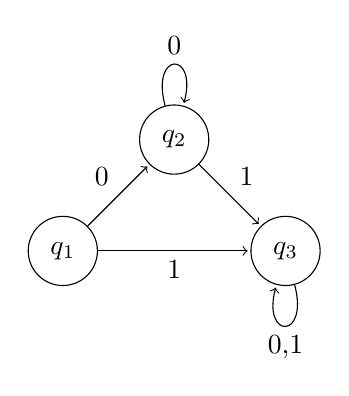
\begin{tikzpicture}[shorten >=1pt,node distance=2cm,on grid,auto] 
  \node[state] (q_1)   {$q_1$}; 
  \node[state] (q_2) [above right=of q_1] {$q_2$}; 
  \node[state] (q_3) [below right=of q_2] {$q_3$}; 
   \path[->] 
   (q_1) edge  node {0} (q_2)
         edge  node [swap] {1} (q_3)
   (q_2) edge  node  {1} (q_3)
         edge [loop above] node {0} ()
   (q_3) edge [loop below] node {0,1} ();
\end{tikzpicture}

By the way, ChatGPT is quite good at outputting tikz code.

\subsubsection{Exploration}

Here are some hints. Why is this material included in the course? What are the big questions that motivate the study of this subject? How does this material connect to broader themes or issues in the field? What practical or theoretical problems can be addressed through an understanding of these topics? A great way to test whether you understand the material is to make your own exercises and answer them. Material related to but going beyond what we do in class is welcome.

Feel free to use your favourite LLM to help you build a mental landscape of the subject. Think of LLMs as an extension of Wikipedia and Google, a tool you should be using as introduction to any subject. If you didn't check with Google, Wikipedia and GPT, you are not ready to write your own notes. On the other hand, while using these resources is necessary, you need to always exercise your own critical thinking and you are always responsible for what you write. 


\subsubsection{Questions}

Ask at least one \textbf{interesting question}\footnote{It is important to learn to ask \emph{interesting} questions. There is no precise way of defining what is meant by interesting. You can only learn this by doing. An interesting question comes typically in two parts. Part 1 (one or two sentences) sets the scene. Part 2 (one or two sentences) asks the question. A good question strikes the right balance between being specific and technical on the one hand and open ended on the other hand. A question that can be answered with yes/no is not an interesing question.} on the lecture notes. Also post the question on the Discord channel so that everybody can see and discuss the questions.

\subsection{Week 2}

Week 2 (and all the other weeks) should follow the same pattern as Week 1, unless instructed otherwise. Even if there is a week without homework, Notes are welcome while Exploration and Questions are still expected.

\subsection{\ldots}

\ldots

\section{Synthesis}

(approx 1 page, plus references)Section 2 gives you an opportunity to practice "skill drill" and to explore the material in more depth. The purpose of this section is to synthesize the knowledge you gained. Since Programming Languages is a wide field, it may be appropriate to focus on a particular topic of your choice. 

We suggest the following timeline. Week 5-8: Decide on a topic and discuss it with your instructor in the office hours. Write a summary email to your instructor after office hours, including the feedback you got with further reflection and planning. Week 9-12: Write a draft of your synthesis and discuss it with your instructor during office hours. Again, write a summary email to your instructor after office hours, including the feedback you got with further reflection and planning. The final version of the Synthesis is due with the rest of the final report.

Here are some example titles you can think of for this section:

\begin{itemize}
\item \textbf{Standard Academic Titles}
  \begin{itemize}
  \item ``Synthesis and Reflection''
  \item ``Integration of Concepts''
  \item ``Synthesis of Learning''
  \item ``Critical Synthesis''
  \end{itemize}

\item \textbf{Algorithm Analysis Focus}
  \begin{itemize}
  \item ``The Core of the Code: A Personal Synthesis''
  \item ``Connecting the Dots: From Theory to Practice''
  \item ``The Big Picture: Algorithm Analysis in Context''
  \item ``Principles of Problem-Solving''
  \end{itemize}

\item \textbf{Concept-Focused Titles}
  \begin{itemize}
  \item ``Beyond the Code: Understanding the Essence of Algorithms''
  \item ``How long is too long? A Case Study in Complexity Theory''
  \item ``Principles of Computation''
  \item ``Abstract Machines for Concrete Problems''
  \item ``Is there an Algorithm for this? On (Un)Decidability''
  \end{itemize}

\item \textbf{Process-Focused Titles}
  \begin{itemize}
  \item ``My Journey Through Algorithm Analysis''
  \item ``From Implementation to Understanding''
  \item ``Building Mental Models of Practical Problems''
  \item ``Discovering the Foundations behind Algorithms''
  \end{itemize}
\end{itemize}


\section{Evidence of Participation}
\section{Conclusion}\label{conclusion}

(approx 400 words) A critical reflection on the content of the course. Step back from the technical details. How does the course fit into the wider world of software engineering? What did you find most interesting or useful? What improvements would you suggest?

\begin{thebibliography}{99}
\bibitem[BLA]{bla} Author, \href{https://en.wikipedia.org/wiki/LaTeX}{Title}, Publisher, Year.
\end{thebibliography}

\end{document}
